\documentclass{article}
\usepackage[utf8]{inputenc}
\usepackage{amssymb}

\title{LELEC2103 : Telecom part, report labvieuw lab 3}
\author{Bronchain Olivier \& Schellekens Vincent }
\date{September 2015}

\usepackage{natbib}
\usepackage{graphicx}
% Répartition
% observation real-ursp: Oli
% observation simulator: Oli
% question pre-lab: Vincent0
% faire le labview de la deuxieme méthode: Vincent ? 

\begin{document}

\maketitle

\section{Pre-Lab}
    \subsection{Question 1 : show that in the absence of noise, $\alpha$ and $\phi$ in Eq. (2) do not have any impact on the maximum output energy solution.}
    The received signal has, in the absence of noise, the following form (given page 53) : 
    \begin{equation}
    y[n] = \sqrt{E_x} \alpha e^{j \phi} \sum_m s[m]g((n-m)T - \tau_d)
    \end{equation}
    
    The maximum output energy solution is the solution to the problem of maximizing $J(\tau) = \mathbb{E}|y(nT+\tau)|^2 = \alpha^2 |e^{j \phi}|^2 E_x * ...$
    
    Because we take the module of $y$, it is straightforward that the $e^{j \phi}$ term of $y$ will vanish, because it's modulus is 1. Also, $\alpha^2$ is just a constant that multiplies the objective function $J$ and it is also clear that is won't affect the solution of the optimization problem.
    
    \subsection{Question 2}
    \subsubsection{What are the two critical assumptions used to formulate the indirect
maximization of the output energy?}
    In the indirect maximization of the output energy, we are searching for local optima (points were the gradient is zero). The solution found by indirect maximization is the global maximum if the global maximum is the only point were the gradient is zero, in other words, there are no local extrema.
    Another critical assumption is that the expectation of the derivative can be approximated by a time average over $P$ symbols.
    \subsubsection{Consider how the presence of the
flat fading channel AWGN can impact this method. Specifically, using
at least one of the critical assumptions, explain how you might mitigate
the impact of these impairments by suitable selection of parameters.}
    The AWGN will distort the results, but if we take the average over a number of symbols $P$ sufficently high (instead of taking the expectation), we should expect to get pretty good results and the effect of the noise will be reduced.
    \subsection{Question 3 : after downsampling a sequence originally sampled at rate $\frac{1}{T_z}$ by a factor $M$, what is the sample period of the resulting signal?}
    Downsampling reduces the sample rate, and we have a new sample rate equal to $\frac{1}{MT_z}$. The sample period is $MT_z$.
    
    
    \subsection{Simulations}
        Now we try to simulate a canal with a delay. The delay had to be choose as $\tau_d = 0,34T_s$ but this didn't gave convenient results so we choose to delay the signal of $\tau_d = 45,34T_s$. Figures \ref{sim} and \ref{plot} contain the results.
\begin{figure}[h]
\centering
\begin{tabular}{|c|c|c|c|}
        \hline
        \texttt{Rx oversampling} & \texttt{Rx sample rate} ($MHz$) & \texttt{error static} (indirect) & \texttt{error static} (direct) \\
        \hline 
        2 & 2 &  17,3& 12,96 \\
        \hline
        4 & 4 &  17,3& 16,81 \\
        \hline
        10 & 10 &  13,39 & 19,36 \\
        \hline
        20 & 20 & 13,39 & 20,25 \\
        \hline
\end{tabular}
\caption{Simulation result for $\tau_d = 45,34T_s$ \label{sim}}
\end{figure}

\begin{figure}[h]
\centering
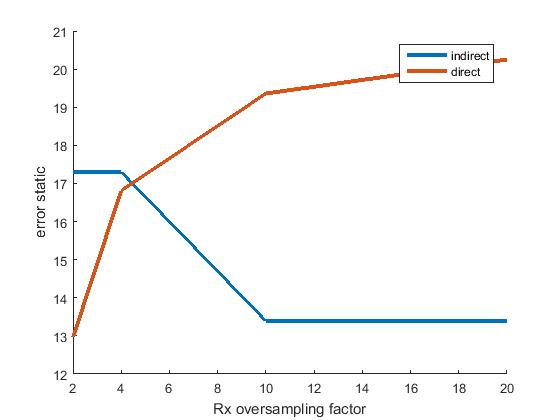
\includegraphics[width = 0.7 \textwidth]{result.jpg}
\caption{\texttt{Error static} vs \texttt{Rx oversampling factor}}
\label{plot}
\end{figure}

We observe that the error increase with the \texttt{Rx sampling factor rate}.

\section{Lab}
    \subsection{Symbol rate}
        The symbol rate ($Sr$) is the number of symbols exchange per seconds. It can be compute as follow:
            $$Sr = \frac{1}{T_s}$$
            $$Sr = \frac{1}{M*dt}$$
            $$Sr = \frac{f_s}{M}$$
        $M$ is the \texttt{RX oversample factor} and $f_s$ is the \texttt{Rx sample rate}. In this case we have:
            $$Sr = \frac{2*10^{6}}{2} = 10^6[symbols/s]$$
        So $10^6$ symbols are exchange per seconds.
        
    \subsection{Variation of N over the constellation}
        We observe the influence of the \texttt{Rx oversample factor} over the constellation and the \texttt{BER} with a fixed \texttt{Tx oversample factor} for the direct and the indirect estimation of the delay. The \texttt{BER} in Figure \ref{obs} are the average bit-error rate over 100 packets for each method. 
        We observe that the \texttt{BER} increase for each method with the \texttt{Rx oversamping factor}. So the constellations get messy when the \texttt{Rx oversampling factor} increase and so for each methods. 
        We also observe that for a few packets, the constellation is more scatter then the other ones even if the parameters don't change. 
        \begin{figure}[h]
        \centering
        \begin{tabular}{|c|c|c|c|}
            \hline
            \texttt{Rx oversample factor} & \texttt{Rx sample rate} & \texttt{BER} (direct) & \texttt{BER} (indirect) \\
            \hline
            2 & 2M & 0,00004 & 0,00038\\
            \hline
            4 & 4M & 0,00018& 0,00082\\
            \hline
            10 & 10M & 0,074 & 0,023688\\
            \hline
            20 & 20M & 0,4653 & 0,462833\\
            \hline
        \end{tabular}
        \caption{Observation on a real wireless link \label{obs}}
        \end{figure}
        \begin{figure}[h]
            \centering
            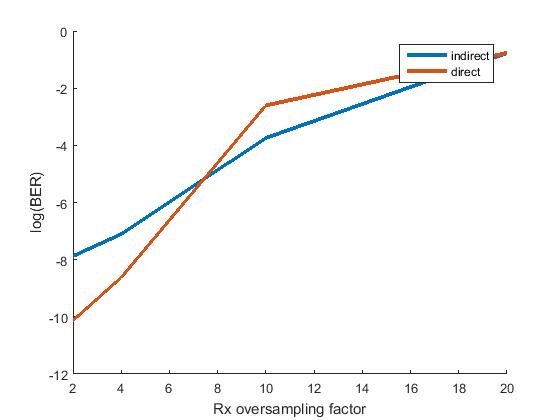
\includegraphics[width = 0.8\textwidth]{logber.jpg}
            \caption{\texttt{BER} vs \texttt{Rx oversampling rate}} 
        \end{figure}
        
        
        \begin{figure}[h]
        \centering
        \begin{tabular}{c c}
        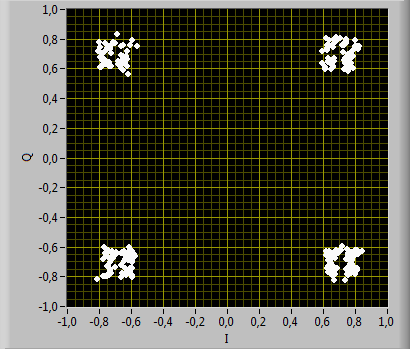
\includegraphics[width = 0.4 \textwidth]{2_2_dir.PNG} & 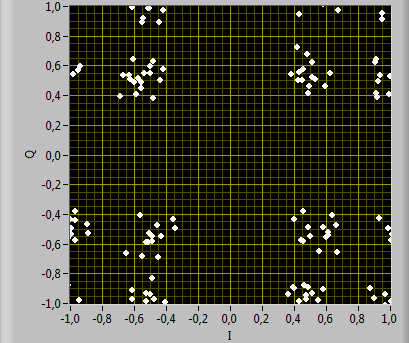
\includegraphics[width = 0.4 \textwidth]{2_2_indir.PNG}\\
        \end{tabular}
        \caption{Signal Constellation for direct and indirect methods with $N=2$ \label{N2}}
        \end{figure}
        
        \begin{figure}[h]
        \centering
        \begin{tabular}{c c}
        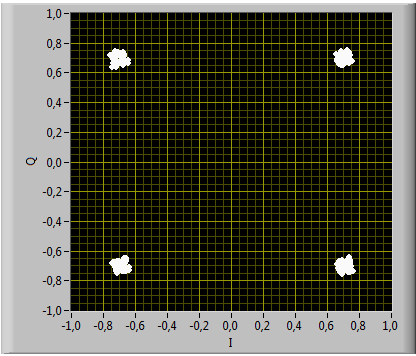
\includegraphics[width = 0.4 \textwidth]{4_4_dir.PNG} & 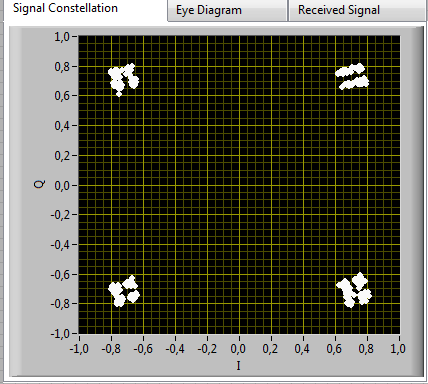
\includegraphics[width = 0.4 \textwidth]{4_4_indir.PNG}\\
        \end{tabular}
        \caption{Signal Constellation for direct and indirect methods with $N=4$ \label{N4}}
        \end{figure}
        
        \begin{figure}[h]
        \centering
        \begin{tabular}{c c}
        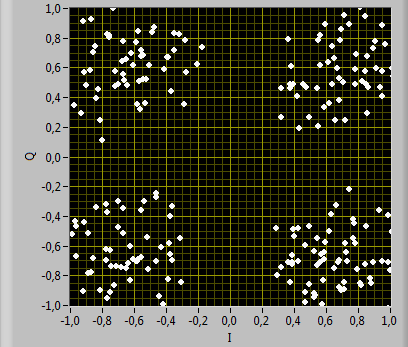
\includegraphics[width = 0.4 \textwidth]{10_10_dir.PNG} & 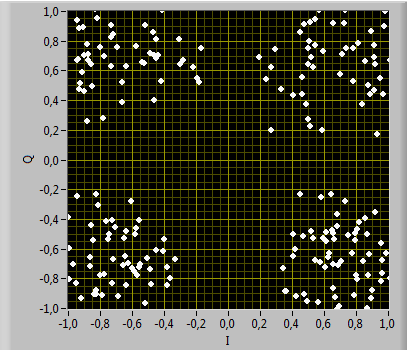
\includegraphics[width = 0.4 \textwidth]{10_10_indir.PNG}\\
        \end{tabular}
        \caption{Signal Constellation for direct and indirect methods with $N=10$ \label{N10}}
        \end{figure}
\end{document}